\section{Introducción}
\subsection{Motivación}
\begin{frame}
 \begin{center}
  \LARGE Motivación
 \end{center}
\end{frame}
\begin{frame}
 \frametitle{Motivación}
 \begin{columns}
  \begin{column}[]{.40\textwidth}
   \begin{figure}[H]
    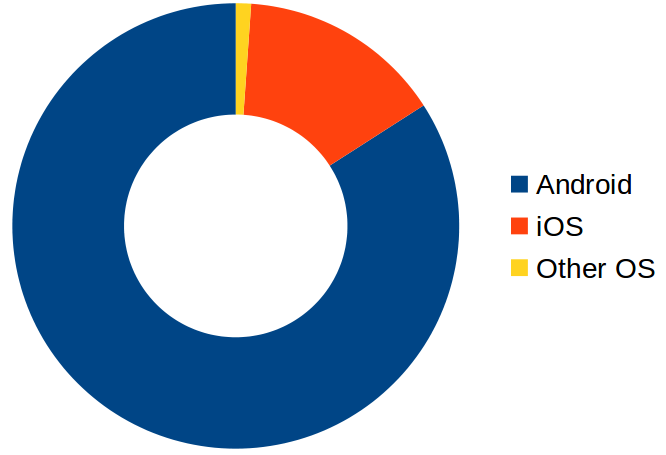
\includegraphics[scale=.15]{imgs/mobile-so-proportion.png} 
    \caption{Ventas mundiales de teléfonos inteligentes a usuarios finales por so.}
    \label{mobile-so}
   \end{figure}
  \end{column}
  \begin{column}[]{.55\textwidth}\pause
   \begin{figure}
     \centering
     \smartdiagramset{bubble node size=3.7cm,
         bubble node font=\tiny , bubble center node font=\tiny
     }
     \smartdiagram[bubble diagram]{
       Android\\más de 3.500.000,iOS\\más de 3.100.000
     }
     \caption{Cantidad de aplicaciones móviles.}
     \label{amount-apps}
   \end{figure}
  \end{column}
 \end{columns}
\end{frame}
\begin{frame}
 \frametitle{Motivación}
 \begin{exampleblock}{Motivación I}
Se incrementan los ataques a los dispositivos móviles, en busca de información personal y confidencial que almacenan, y de las operaciones realizadas a través de ellos.
  \end{exampleblock}
  \pause
  \begin{exampleblock}{Motivación II}
Debido al uso diario de estas aplicaciones, se puede filtrar una gran cantidad de información privada y confidencial.
   \end{exampleblock}
\end{frame}

\subsection{Modelo de Android}
\begin{frame}
 \begin{center}
  \LARGE Modelo de Android
 \end{center}
\end{frame}
\begin{frame}
 \frametitle{Modelo de Android}
 {Android es un sistema operativo de código abierto, diseñado para dispositivos móviles y desarrollado por Google junto con la Open Handset Alliance.}\pause
 \begin{figure}[H]
    \centering
    \begin{subfigure}{0.75\linewidth}
		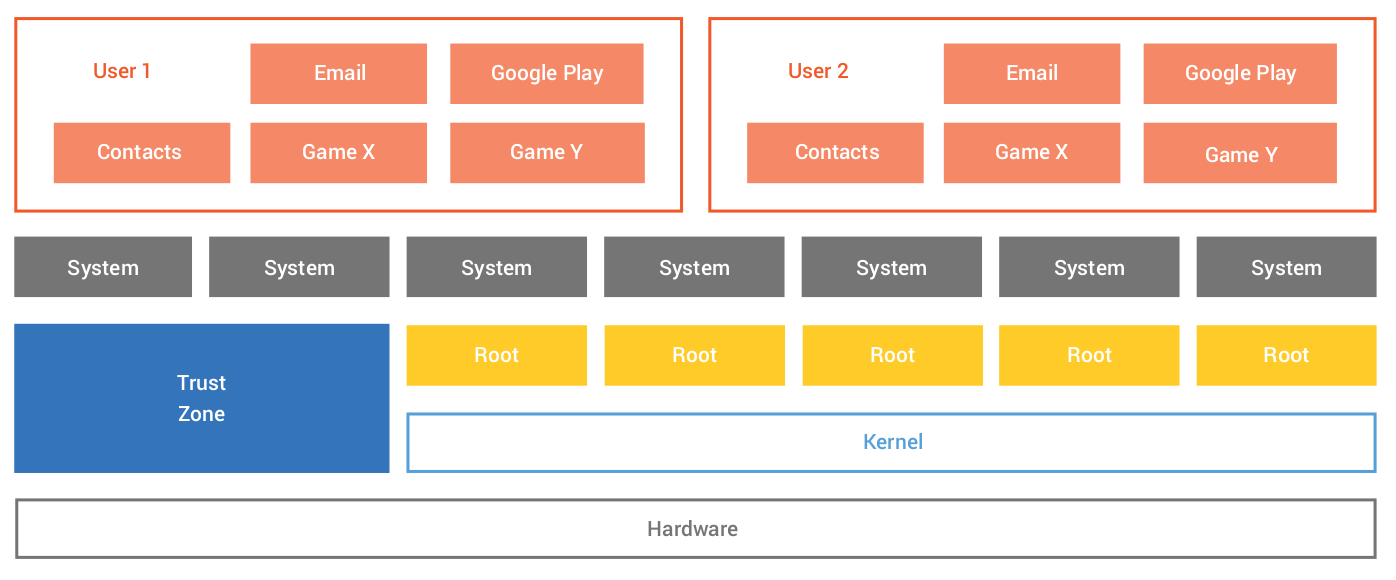
\includegraphics[width=\linewidth]{android_security_model}
	    \label{fig:ch01:sandbox}
    \end{subfigure}
    \caption{Aislamiento de las aplicaciones según su UID.}
 \end{figure}
\end{frame}
\begin{frame}
 \frametitle{Modelo de Android}
 \begin{small}
 \begin{itemize}
     \item Podemos clasificar los permisos según el riesgo implícito al otorgarlos:
     \begin{multicols}{2}
     \begin{itemize}[<+->]\small
      \item \emph{\textbf<5->{Normal}}
      \item \emph{\textbf<5->{Dangerous}}
      \item \emph{\invisible<5->{Signature}}
      \item \emph{\invisible<5->{Signature/System}}
     \end{itemize}
     \end{multicols}\pause
     \item A partir de la versión 6.0 se propone un nuevo modelo de permisos:\pause
         \begin{figure}[btp]
            \begin{subfigure}{0.4\linewidth}
            \centering
                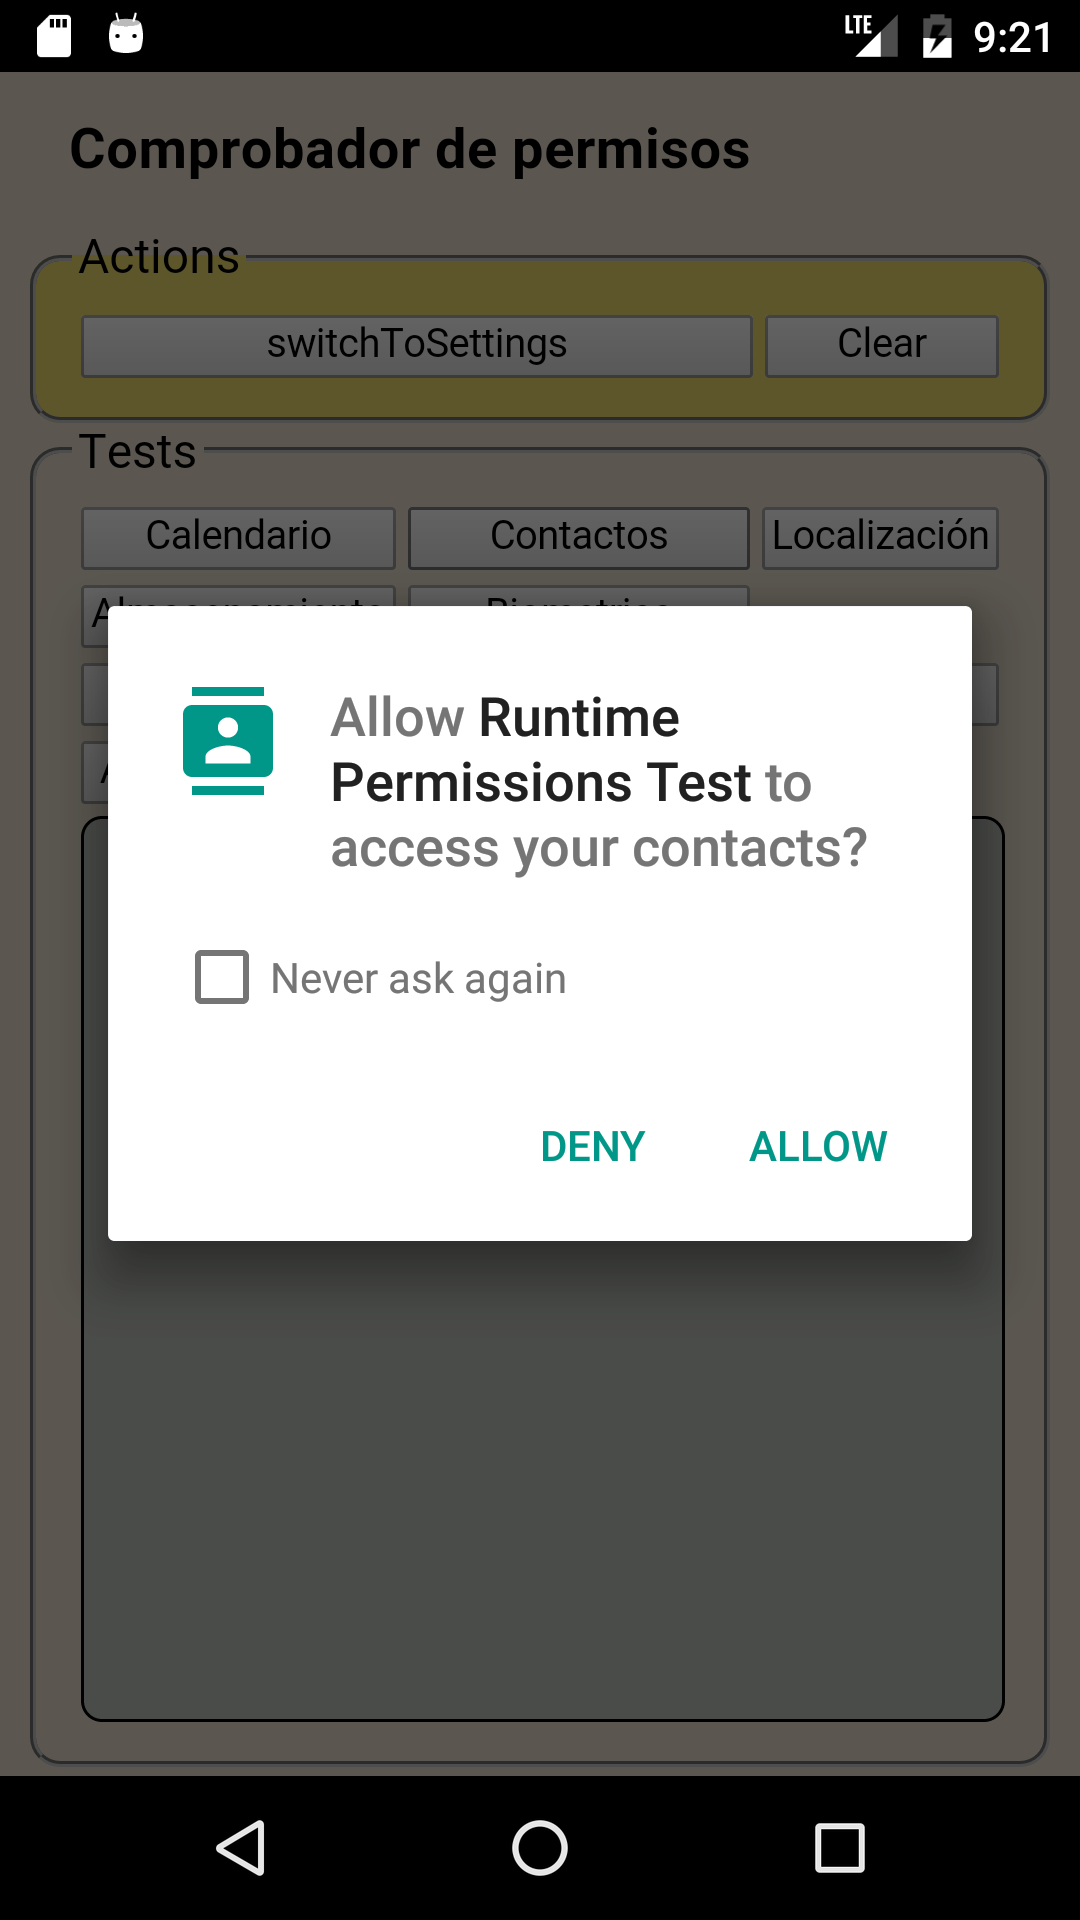
\includegraphics[width=.5\linewidth]{allow_contact}
                \caption{Solicitud de un permiso.}
            \end{subfigure}
        \begin{subfigure}{0.4\linewidth}\pause
        \centering
            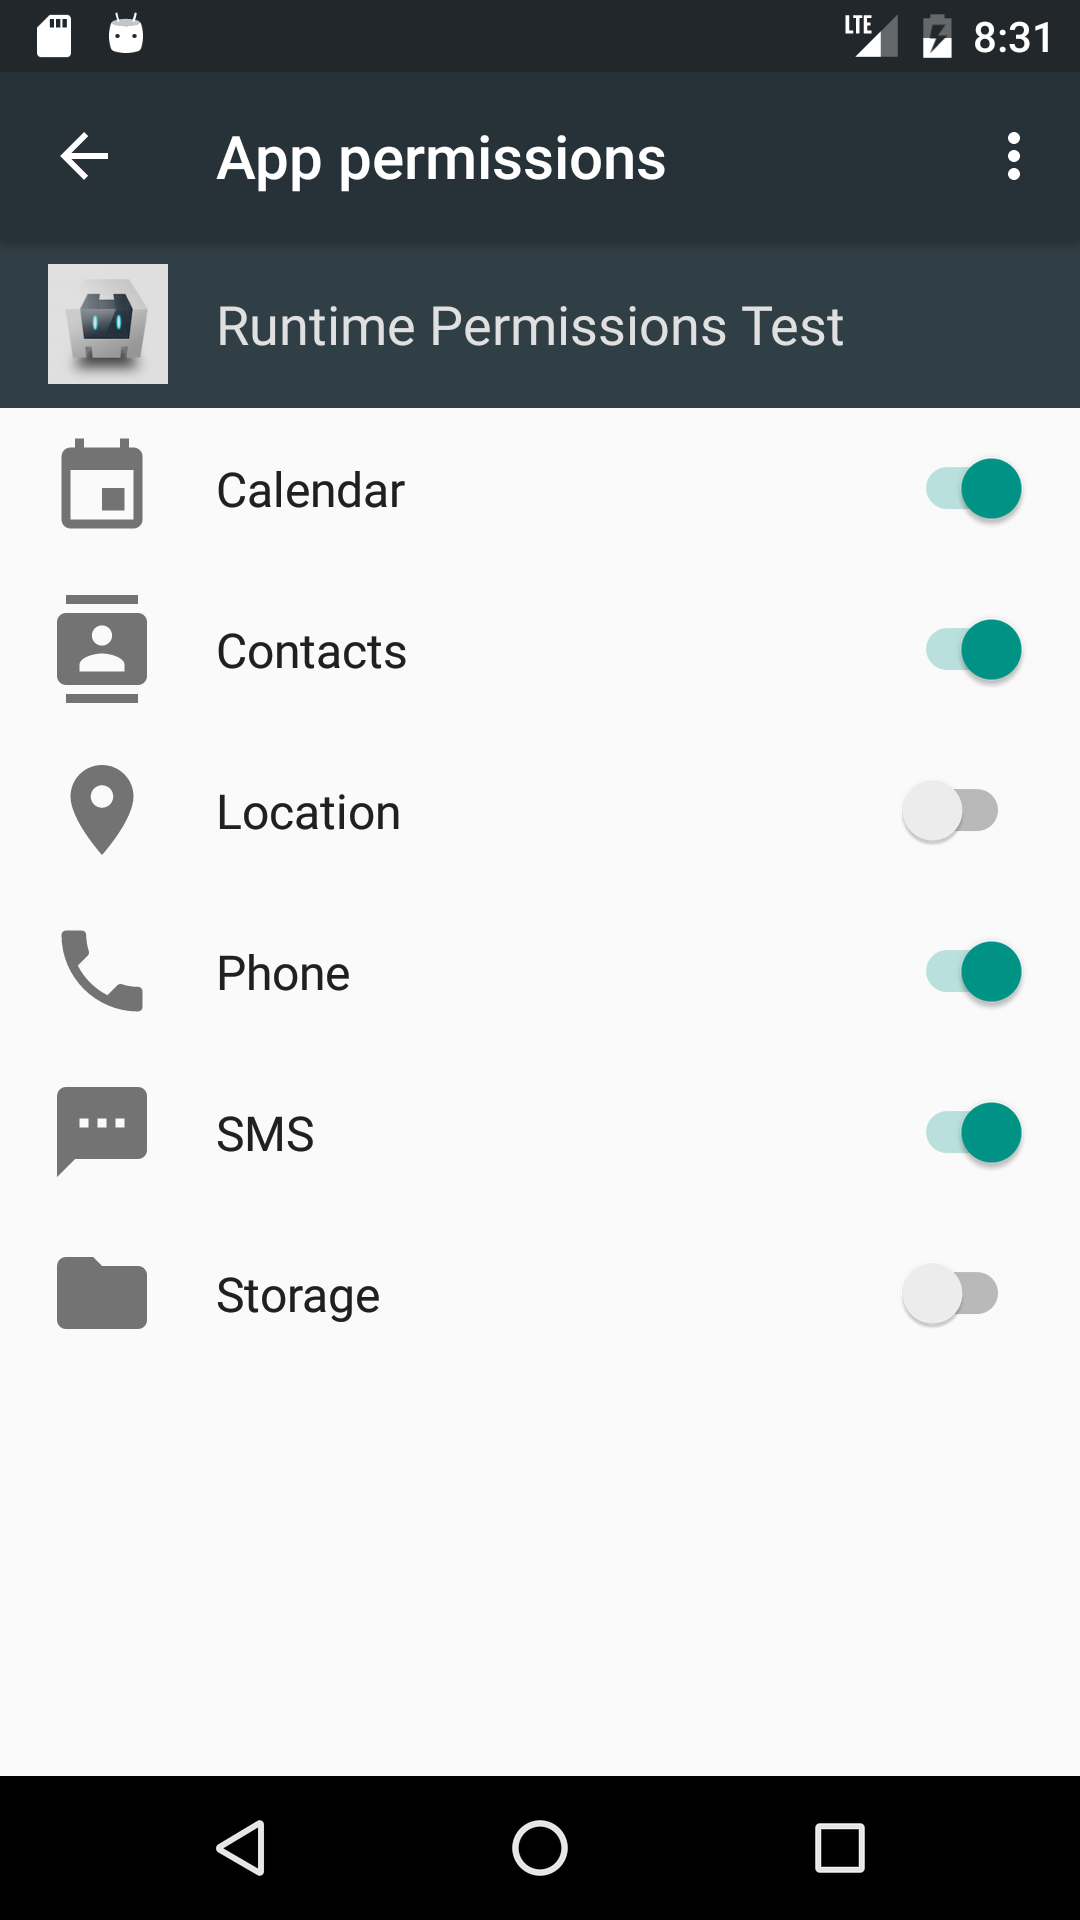
\includegraphics[width=.5\linewidth]{app-permissions}
            \caption{Listado de los permisos.}
    	\end{subfigure}
    	\caption{Nuevo modelo de permisos.}
        \end{figure}
 \end{itemize}
  \end{small}
\end{frame}

\subsection{Modelo de iOS}
\begin{frame}
 \begin{center}
  \LARGE Modelo de iOS
 \end{center}
\end{frame}
\begin{frame}
 \frametitle{Modelo de iOS}
 \begin{figure}[tH]
  \begin{subfigure}{0.7\linewidth}
   \begin{itemize}
    \item iOS es un sistema operativo para dispositivos móviles de la multinacional Apple Inc. diseñado para ser
seguro. \pause
    \item Las principales características de seguridad no son configurables y vienen habilitadas por defecto.
   \end{itemize}
  \end{subfigure}
  \begin{subfigure}{0.25\linewidth}\pause
    \centering
    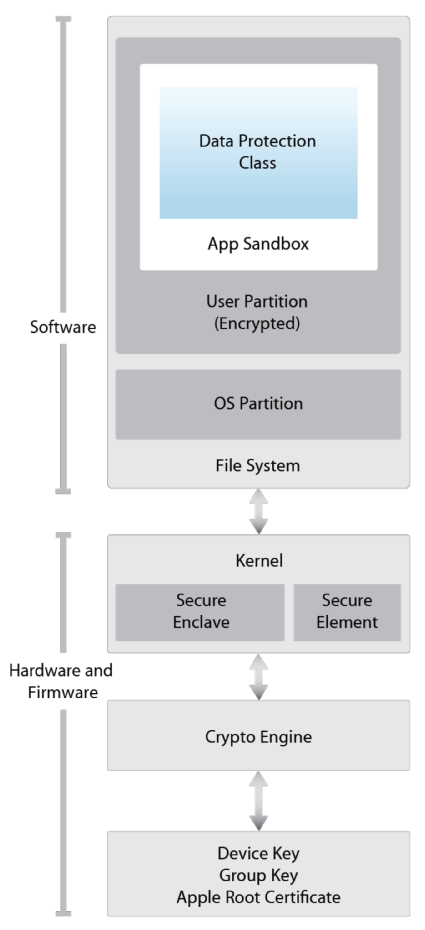
\includegraphics[width=\linewidth]{ios_security_architecture}
  \end{subfigure}
  \caption{Entorno seguro de iOS.}
\end{figure}
\end{frame}
\begin{frame}
 \frametitle{Modelo de iOS}
 \begin{itemize}
  \item Las aplicaciones pueden solicitar un permiso solamente mientras se esté ejecutando. \pause
 \end{itemize}
 \begin{figure}[hbtp]
    \centering
    \begin{subfigure}{0.49\linewidth}
    \centering
    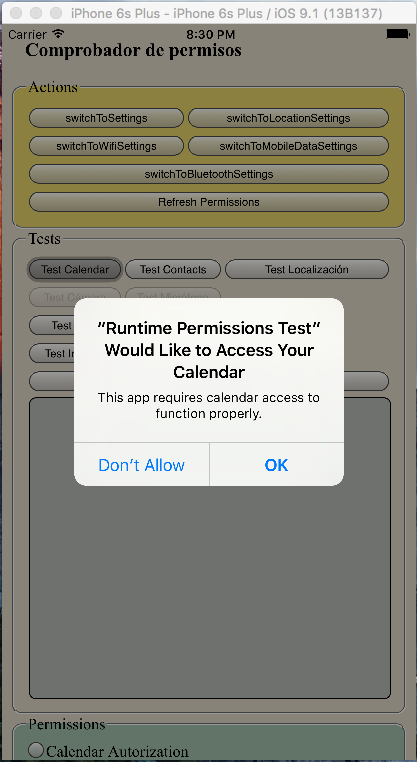
\includegraphics[width=.5\linewidth]{calendar_request_ios}
    \caption{Solicitud de un permiso.}
    \end{subfigure}
    \begin{subfigure}{0.49\linewidth}
    \centering
     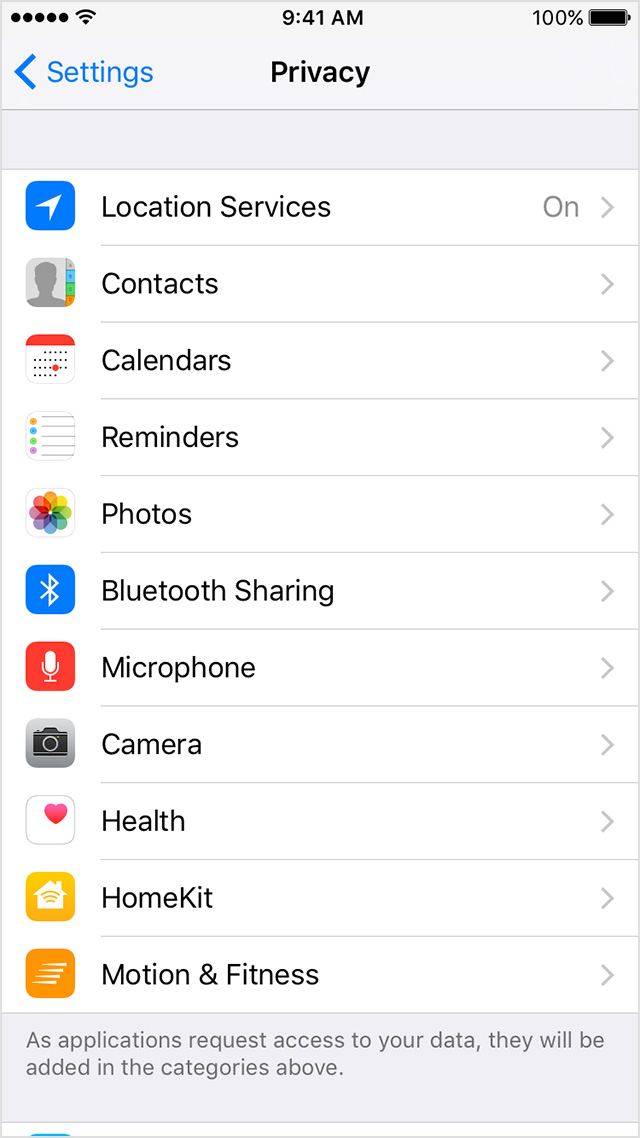
\includegraphics[width=.5\linewidth]{settings-privacy}
    \caption{Control de privacidad.}
    \end{subfigure}
    \caption{Sistema de permisos de iOS 9.}
 \end{figure}
\end{frame}

